\documentclass[a4paper,11pt,titlepage]{article}
\usepackage{amssymb}
\usepackage{hyperref}
\usepackage{booktabs}
\usepackage{geometry}
\usepackage{listings}
\usepackage{graphicx}
\usepackage{natbib}
\usepackage{todonotes}
\usepackage{enumitem}
\usepackage{multirow}
\usepackage{tikz}
\usepackage{fancyhdr}
\usetikzlibrary{arrows,decorations.pathmorphing,backgrounds,positioning,fit,petri,matrix,folding}

\setlength\headheight{20pt}
\addtolength\topmargin{-10pt}
\addtolength\footskip{20pt}

\fancypagestyle{plain}{%
\fancyhf{}
\fancyfoot[RO,LE]{\sffamily\bfseries\thepage}
\renewcommand{\headrulewidth}{0pt}
\renewcommand{\footrulewidth}{1pt}
}


\newcommand{\HRule}{\rule{\linewidth}{0.5mm}}

\newcommand{\uni}{Eindhoven University of Technology}
\newcommand{\fase}{Computer Science and Engineering}
\newcommand{\vak}{Business Process Simulations}
\newcommand{\vakcode}{2II75}
\newcommand{\essaytitle}{Large Fuel Station Analysis}
\newcommand{\stad}{Eindhoven}
\newcommand{\tbsep}{\ \ \textbar \ \textbar \ \textbar \ \textbar \ \textbar \ \textbar \ \textbar \ \textbar \ \textbar \ \textbar \ \ }

\pagestyle{fancy}
\fancyhf{}
\fancyhead[RO,LE]{\vak}
\fancyhead[LO,RE]{\uni}
\fancyfoot[RO,LE]{\sffamily\bfseries\thepage}
\fancyfoot[LO,RE]{\essaytitle}
\renewcommand{\headrulewidth}{1pt}
\renewcommand{\footrulewidth}{1pt}

\bibliographystyle{plain}
\hypersetup{pdfborder={0 0 0}}

\setlength{\parskip}{10pt}

\geometry{
	includeheadfoot,
	margin=2.54cm
}
\author{
	Nicky Advokaat (0740567) - \texttt{n.advokaat@student.tue.nl}
	\and
	Robbert Jongeling (0747896) - \texttt{r.m.jongeling@student.tue.nl}
	\and
	Bram Kohl (0746107) - \texttt{b.j.e.kohl@student.tue.nl}
	\and
	Jasper Selman (0741516) - \texttt{j.w.m.selman@student.tue.nl}
	\and
	Ramon de Vaan (0758873) - \texttt{r.d.vaan@student.tue.nl}
}
\date{\today}

\begin{document}
	\begin{titlepage}
	\begin{center}

% Upper part of the page
		
\includegraphics[width=0.15\textwidth]{images/tuelogo}\\[1cm]

		\textsc{\LARGE \uni}\\[0.2cm]

		\textsc{\fase}\\[1.6cm]

        \textsc{\LARGE \vak}\\[0.5cm]

% Title
\HRule \\[0.4cm]
{ \huge \bfseries \essaytitle}\\[0.4cm]

\HRule \\[1.5cm]

% Author and supervisor
	\emph{Group 13:}\\
    \begin{tabular}{l l l}
	Nicky \textsc{Advokaat} & 0740567 & \href{mailto:n.advokaat@student.tue.nl}{\texttt{n.advokaat@student.tue.nl}}\\
	Robbert \textsc{Jongeling} & 0747896 & \href{mailto:r.m.jongeling@student.tue.nl}{\texttt{r.m.jongeling@student.tue.nl}}\\
	Bram \textsc{Kohl} & 0746107 & \href{mailto:b.j.e.kohl@student.tue.nl}{\texttt{b.j.e.kohl@student.tue.nl}}\\
	Jasper \textsc{Selman} & 0741516 & \href{mailto:j.w.m.selman@student.tue.nl}{\texttt{j.w.m.selman@student.tue.nl}}\\
	Ramon \textsc{de Vaan} & 0758873 & \href{mailto:r.d.vaan@student.tue.nl}{\texttt{r.d.vaan@student.tue.nl}}
    \end{tabular}
		\vfill

% Bottom of the page
		{\large \today} \\
		\stad

	\end{center}
\end{titlepage}
    \tableofcontents
    \listoftables
    \listoffigures
    \newpage
	\section{Executive Summary}
Bill Perterson of BP fuel wants to open a new large fuel station. He has a problem with creating a cashier schedule for the pumps, such that his profit is maximized but the schedule also meets the following requirements:
\begin{enumerate}
\item Cars (with  trailers) typically spend at most 30 minutes from arrival to departure.
\item Trucks typically spend at most 45 minutes from arrival to departure.
\item At most 1$\%$ of the arriving vehicles will be blocked.
\end{enumerate}
    \newpage
	Despite the rapid depletion of fossil fuel resources, and the rise of the electric vehicle industry, the fuel station industry remains big business.
As a result, Bill Peterson of BP fuel is opening a new, very large fuel station in Luxemburg.
Bill has a specific layout in mind: the fuel station will have 15 fuel pumps divided in 5 groups of 3 pumps each.
Every group will have a single cashier.
Vehicles will queue in one of the 15 lanes and wait for their turn at the pump.
Afterwards, they will head to the associated cashier to pay.

Since Bill lacks experience in scheduling the workers in the specified fuel station layout, we, group 13, have been hired as a consultant to tackle that problem.
Obviously, our goal is to maximize the profit of the fuel station, whilst satisfying several requirements made by Bill regarding customer satisfaction.
We are, however, limited in certain aspects.
First of all, fuel prices are fixed in Luxembourg, so we cannot reduce or increase prices to either get more customers or increase profit per customer.
As a result, the only way for us to increase the profit, is to reduce the cost of the fuel station, by changing the schedule of the workers.
Luckily, Bill has collected many statistics about vehicles entering one of his competitor's fuel stations and has recorded information about fuel amounts in some of his other fuel stations.

In this report we will analyse the problem described above, to provide a base on which we will later deliver a recommendation regarding not only the current situation, but possible future situations, if his needs were to change.
We will attempt to do so, firstly by describing the system in detail, making assumptions on things that were not explained fully.
Next, we will analyse the input provided to us, trying to fit statistical models to the data.
Finally, we will provide conceptual models by all group members individually.
	
	\section{System Description}
In this section we give a description of the fuel station.
First, we describe all key object classes appearing in the model and their associated actions. 
Next, performance indicators are listed.
Thirdly, we pose questions to be answered by our research.
Finally, we name alternative solutions to achieve Bills goals.

\subsection{Key Object Classes}
In our fuel station we can distinguish several key object classes.
Table \ref{tab:koc} shows all key object classes as well as their types and states.
The classes we distinguish are \textit{Vehicle}, \textit{Lane}, \textit{Employee}, \textit{Pump} and \textit{Queue Spot}. 

The class \textit{Vehicle} consists of three types: \textit{Car, Car with Trailer} and \textit{Truck}.
 Vehicles are in one of six states while they are in the fuel station. 
 The first state is \textit{Arriving}, a vehicle in this state has entered the fuel station but has not yet chosen any queue to enter.
 A vehicle in the next state, \textit{In Queue}, has chosen a queue and is waiting in line. 
 The third state, \textit{Refueling}, indicates that the vehicle has reached the pump and is now refueling. 
 The fourth state, \textit{Waiting for Cashier} means the vehicle is done refueling, but has not reached the cashier yet. 
 The next state, \textit{Paying}, means the vehicle has reached the cashier and payment is being handled. 
 When a vehicle is in the last state, \textit{Idle}, it has outside our station i.e. it has not yet arrived or has already left.
 
The second class is \textit{Lane}, it consists of a single type, also named \textit{Lane}.
A \textit{Lane} is a queue in front of the pumps and is in one of two states. 
The first state is \textit{Available}, i.e. vehicles can enter the lane.
The second state is \textit{Closed}, i.e. no vehicle can enter the lane.
We assume that within groups of three lanes, the state is shared, i.e., in every group either all lanes are opened or all lanes are closed.

The third class is the \textit{Employees}, in this model we consider only one type of employee, \textit{Cashier}. 
A cashier can be in one of four states.
The first state is \textit{Off-duty}, i.e. the cashier is not working at the moment. 
Secondly, there is the state \textit{Available}, the cashier is on duty but he is not serving customers at the moment. 
When he is busy serving a customer he is in the third state, \textit{Serving}.
The last state a cashier can be in is the state \textit{Restocking Supplies}. 
This means the shift of the cashier has ended but he is restocking the supplies.

The fourth class is \textit{Pump}.
Each of these pumps can be either in the \textit{Available} or \textit{In Use} state.
We assume that each pump is capable of providing fuel at low and high speed, depending on the vehicle type.
Furthermore we assume that there is enough fuel stored to ensure a continuous flow.

The last class is \textit{Queue Spot}. 
This class represents the spots which are available between the pumps and the cashier. 
There are three kinds of spots. 
\textit{First Spot} is the spot right after the pump and there are three of them for every group of three lanes a served by a single cashier.
\textit{Second  Spot} is the spot after \textit{First Spot} and there are only two of them for every group of three lanes. 
\textit{Third Spot} is the last spot and also the spot where a vehicle is served by a cashier, there is only one of them for every group of three lanes. 
Every one of these spots can either be occupied by a vehicle or be free, hence the states \textit{Occupied} and \textit{Free}.

\begin{center}
\begin{table}[h]
\begin{tabular}{| l | l | l | l | l |}
\hline
\textbf{Vehicle} & \textbf{Lane} & \textbf{Employee} & \textbf{Pump} & \textbf{Queue Spot}\\
\hline
\textbf{Types} & \textbf{Types} & \textbf{Types} & \textbf{Types} & \textbf{Types}\\
- Car & - Lane & - Cashier& & - First Spot\\
- Car with Trailer & & & & - Second Spot\\
- Truck & & & & - Third Spot\\
& & & & \\
\textbf{States} & \textbf{States} & \textbf{States} & \textbf{States} & \textbf{States}\\
- Arriving & - Available & - Off-duty & - Available & - Free\\
- In Queue & - Closed & - Available & - In Use & - Occupied\\
- Refueling & & - Serving & &\\
- Waiting for Cashier & & - Restocking Supplies & &\\
- Paying & & & &\\
- Idle & & & &\\
\hline
\end{tabular}
\caption{Key Object Classes}
\label{tab:koc}
\end{table}
\end{center}

\subsection{Actions}
We model six actions that occur in the system.
Each of these actions causes a number of state changes, depending on the state the system is in when the action occurs. 
Below we enumerate these actions along with the state changes they cause.

\begin{enumerate}
	\item \textbf{A vehicle arrives}
	\begin{enumerate}
		\item Vehicle state changes from \textit{Idle} to \textit{Arriving}.
		\item If every lane is either \textit{Closed} or there is insufficient space for the arriving vehicle, then the vehicle becomes \textit{Idle} again.
		\item If a lane is \textit{Available} and the Pump is \textit{Available} (No Vehicle using or blocking it) then:
	\begin{enumerate}
		\item The Pump goes from \textit{Available} to \textit{In Use}.
		\item The Vehicle goes from \textit{Arriving} to \textit{Refueling}
	\end{enumerate}
	Assumption: If a Pump is \textit{Available}, the Lane is empty (i.e. when a Vehicle stops blocking it, the next Vehicle starts using it at the same time).
	\item If a lane is \textit{Available} and there is enough space for the arriving Vehicle and the Pump is \textit{In Use} then the Vehicle goes from \textit{Arriving} to \textit{In Queue}
	\end{enumerate}
	
	\item \textbf{A cashier starts a shift}
	\begin{enumerate}
		\item If there is no Vehicle at the Third Queue Spot of the Cashier, the Employee goes from \textit{Off-duty} to \textit{Available}.
		\item If there is a Vehicle at the Third Queue Spot of the Cashier, the Employee goes from \textit{Off-duty} to \textit{Serving}.
		\item If the Lanes the cashier is working on are \textit{Closed}, they change to \textit{Available}.
	\end{enumerate}
	
	\item \textbf{A cashier's regular shift ends}
	\begin{enumerate}
		\item If another cashier takes over, the Employee whose shift ends goes from \textit{Available} or \textit{Serving} to \textit{Restocking Supplies}
		\item If no cashier takes over then
		\begin{enumerate}
			\item The Lanes of the cashier go from \textit{Available} to \textit{Closed}
			\item If the Lane and the Queue Spots are empty, the Employee goes from \textit{Available} to \textit{Restocking Supplies}
		\end{enumerate}
	\end{enumerate}
	
	\item \textbf{A cashier finishes Restocking Supplies}
	\begin{enumerate}
		\item{The Employee goes from \textit{Restocking Supplies} to \textit{Off-duty}}
	\end{enumerate}
	
	\item \textbf{A vehicle finishes refueling}
	\begin{enumerate}
		\item If there are \textit{Free} Queue Spots the Vehicle can move to, the Queue Spots go from \textit{Free} to \textit{Occupied}
		\item If the Vehicle can move completely to the Queue Spots of the cashier, and there is a Vehicle waiting in the Lane then the waiting Vehicle goes from \textit{In Queue} to \textit{Refueling}
		\item If the Vehicle can move completely to the Queue Spots of the cashier and there is no Vehicle waiting in the Lane, the Pump goes from \textit{In Use} to \textit{Available}.
		\item If the cashier of the Lane the Vehicle is in is \textit{Available} then:
		\begin{enumerate}
			\item The Vehicle goes from \textit{Refueling} to \textit{Paying}
			\item The Employee of the Lane the Vehicle is in goes from \textit{Available} to \textit{Serving}
		\end{enumerate}
		Assumption: If the cashier is \textit{Available}, there are no Vehicles in his Queue Spots (i.e. when an Employee would become \textit{Available} with Vehicles in his Queue Spots, he becomes/stays \textit{Serving} instead).
		\item If the cashier of the Lane the Vehicle is in is \textit{Serving}, then the Vehicle goes from \textit{Refueling} to \textit{Waiting for Cashier}.
		%If lane can be blocked, check if it can be unblocked here
	\end{enumerate}
	
	\item \textbf{A vehicle has payed}
	\begin{enumerate}
		\item The Vehicle goes from \textit{Paying} to \textit{Idle}.
		\item If there are Vehicles in the Queue Spots of the cashier then:
		\begin{enumerate}
			\item One of those Vehicles changes from \textit{Waiting for Cashier} to \textit{Paying}
			\item If a Vehicle can move further in the Queue Spots causing a Pump to no longer be blocked, then that Pump goes from \textit{In Use} to \textit{Available}
			\item If Queue Spots open up due to Vehicles moving, they go from \textit{Occupied} to \textit{Free}
		\end{enumerate}
		\item If there are no Vehicles in the Queue Spots of the cashier, then the Employee goes from \textit{Serving} to \textit{Available}
		\item If the Lanes of the cashier are \textit{Closed} and the \textit{Queue Spots} of the cashier are all \textit{Free}, and if less than 10 minutes passed since the cashier's regular shift ended the Employee goes from \textit{Serving} to \textit{Restocking Supplies}. 
		\item If the Lanes of the cashier are \textit{Closed} and the \textit{Queue Spots} of the cashier are all \textit{Free}, and if at least 10 minutes passed since the cashier's regular shift ended, the Employee goes from \textit{Serving} to \textit{Off-duty}. 
	\end{enumerate}
\end{enumerate}

\subsection{Performance Indicators:}
We consider two performance indicators.
First, we consider average throughput time i.e. the time between arriving and leaving of a car or truck.
This time should be at most 30 minutes for cars and cars with trailers and at most 45 minutes for trucks.
The second performance indicator is the cost of the staffing schedule.
As mentioned in the assignment, having 5 cashiers on duty at all times costs about 3200 euro per day.


\subsection{Questions to be answered}
There are two questions that our simulation study needs to answer. 
The most important question is: "\textit{What is the most cost effective cashier schedule that satisfies the customer requirements?}". 
The second question is \textit{How should the cashier schedule be adopted to the expected decreases in customer demand?}", since vehicles are becoming more and more fuel-efficient.

These questions can be divided in sub-questions, "\textit{What should be the expected waiting times for trucks and cars?}" and "\textit{What is the percentage of blocked vehicles entering the fuel station?}". 
Another question is \textit{"What is the required number of cashiers per shift?}"
These are all questions which can be used to answer the first question. 
To answer the second question we can in fact use the same sub-questions, we only need different data, since the number of arrivals are very different. 

	
	\section{Input Analysis}
A histogram of the number of arrivals over time is shown in Figure \ref{fig:histogram-arrivals}. 
Fitting analysis has shown that a Beta distribution is the best fit for this data, a summary of the Fit all functionality of Arena Input Analyzer is shown in Table \ref{tab:fitallarrivals}.

\begin{figure}[h]
	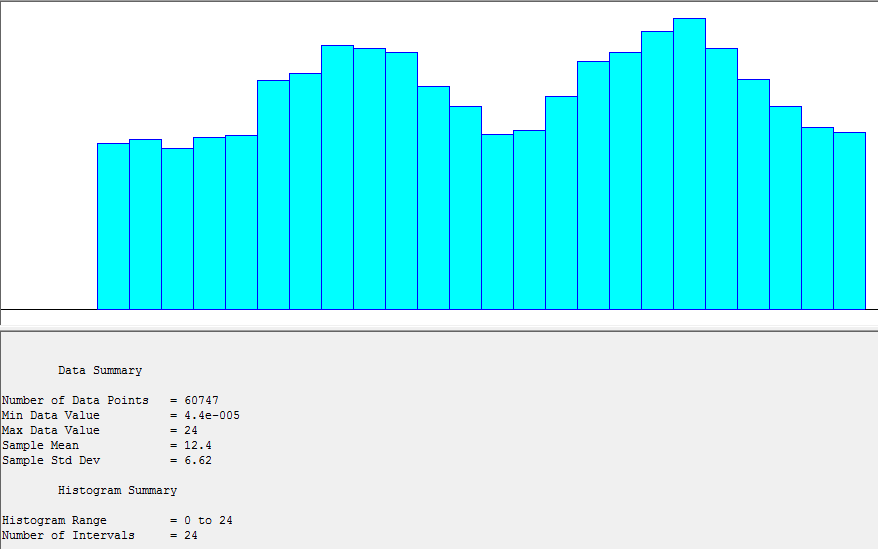
\includegraphics[width=\textwidth]{images/histogram-arrivals.PNG}
	\caption{Histogram of arrival times, each of the 24 intervals represents one hour.}
	\label{fig:histogram-arrivals}
\end{figure}

\begin{table}[h]
	\centering
	\begin{tabular}{r | l}
		Function  &     Sq Error\\
		\hline
		Beta       &  0.000889\\
		Uniform     & 0.00141\\
		Normal       &0.00507\\
		Gamma        &0.00703\\
		Erlang       &0.00712\\
		Triangular   &0.00915\\
		Lognormal    &0.0122\\
		Exponential  &0.0143\\
		Weibull      &0.107	
	\end{tabular}
	\caption{Fit all summary of Arena Input Analyzer on Arrivals\_(13).dst}
	\label{tab:fitallarrivals}
\end{table}

In the fuel amounts dataset, we see a clear difference between cars and trucks.
A histogram of the fuel amounts is shown in Figure \ref{fig:histogram-amounts-unfiltered}, here the high peak corresponds to fuel needed by cars, the lower bars correspond to fuel needed by trucks.
In Figure \ref{fig:histogram-amounts-filtered}, a histogram is shown of only the car data, here the maximum data value has been set to 100.
In Table \ref{tab:fitallamounts} summaries of \textit{Fit all} of the Arena Input Analyzer are shown.
The car data in itself is best described by a normal distribution, all data is best described by a Lognormal distribution, where all car data is compressed into one bar of the histogram.

\begin{figure}[h]
	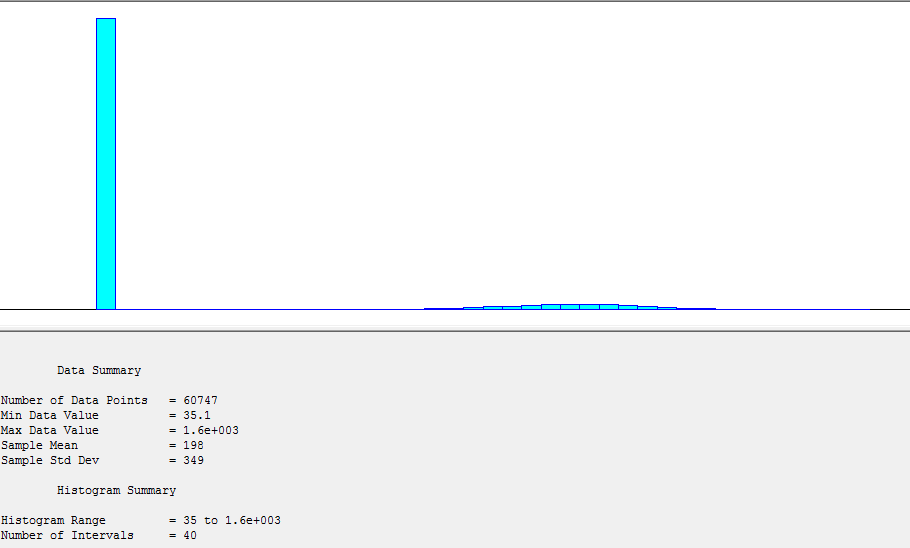
\includegraphics[width=\textwidth]{images/histogram-amounts-unfiltered.PNG}
	\caption{Histogram of used fuel amounts, 40 intervals, on the raw data}
	\label{fig:histogram-amounts-unfiltered}
\end{figure}

\begin{figure}[h]
	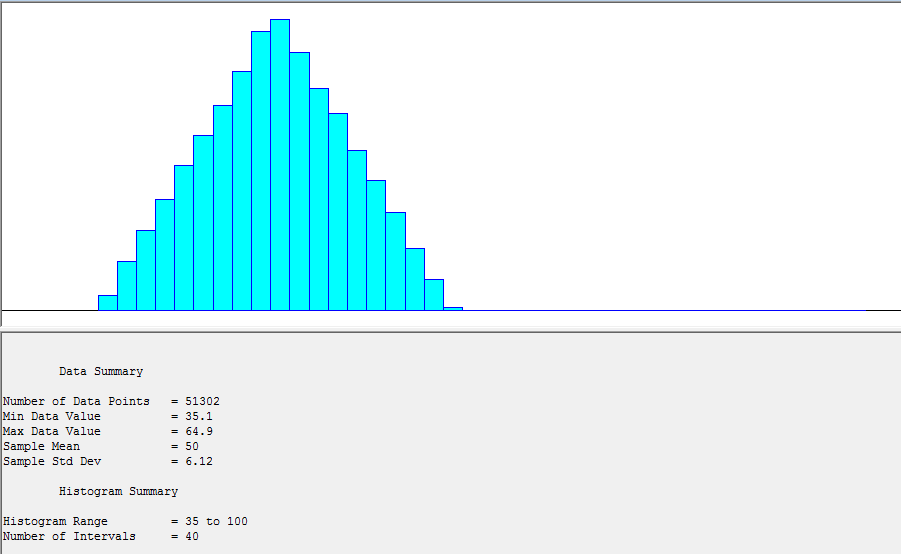
\includegraphics[width=\textwidth]{images/histogram-amounts-filtered.PNG}
	\caption{Histogram of used fuel amounts, 40 intervals, when maximum data value was set to 100 litres.}
	\label{fig:histogram-amounts-filtered}
\end{figure}

\begin{table}[h]
	\parbox{.45\linewidth}{
		\centering
		\begin{tabular}{r | l}
			Function  &     Sq Error\\
			\hline
			Lognormal    &0.0976\\
			Weibull      &0.118\\
			Beta         &0.226\\
			Gamma        &0.285\\
			Exponential  &0.473\\
			Erlang       &0.473\\
			Normal       &0.668\\
			Triangular   &0.679\\
			Uniform      &0.69\\
		\end{tabular}
		\caption{Fit all summary of Arena Input Analyzer on Amounts\_(13).dst}
		\label{fitallamountsunfiltered}
	}
	\parbox{.1\linewidth}{\ }
	\parbox{.45\linewidth}{
		\centering
		\begin{tabular}{r | l}
			Function  &     Sq Error\\
			\hline
			Normal       &0.000575\\
			Weibull      &0.000587\\
			Beta         &0.00239\\
			Erlang       &0.00387\\
			Gamma        &0.00411\\
			Lognormal    &0.00888\\
			Triangular   &0.0277\\
			Exponential  &0.0397\\
			Uniform      &0.0471\\
			
		\end{tabular}
		\caption{Fit all summary of Arena Input Analyzer on Amounts\_(13).dst with maximum amount set to 100}
				\label{fitallamountsfiltered}
	}
	\caption{Summaries of \textit{Fit all} of Arena Input Analyzer}
	\label{tab:fitallamounts}
\end{table}




	
    \section{Simulation Model Description}

In this section the Arena model is described and explained. The model has been split into two models, firstly the management of the cashiers (main model) and secondly the management of the vehicles (submodel Pumps). The used variables, attributes and schedules will be described as well.

\subsection{Cashier management}
First we describe this model such that it is known what this model does and how it works but not the details how this works. The details will be described after that. In fact what this model does is that it creates five checkouts at the start. These checkouts are the entities which go through the system. When cashiers arrive they are put in a set of available cashiers and the checkouts seize a cashier. When a cashier is seized the checkout opens its associated lanes for 4 hours and after that it is decided if another cashier takes over the checkout or if the checkout closes. If it closes all the vehicles currently in the lane will be served and and then the cashier leaves. If another cashier takes over the checkout the old cashier restocks the supplies and goes home. Just before the cashier finishes its shift a duplicate of the checkout is created, since the old entity of this checkout leaves the system after the shift. The duplicate behaves the same as the old entity and the model continues with still five checkouts. A figure of the complete cashier management model can be found in figure \ref{fig:model-cashier} in appendix \ref{app:modeldescription}.

Now lets discuss the model in more detail with figures. We will handle each different module on the figure. The first part of the model is shown in  figure \ref{fig:createcheckouts}. The first module is $Create \ Checkout$. This module creates at the start of every simulation five checkouts. These checkouts are assigned a number from 1 to 5 in the next module, $Assign \ checkout \ numbers$, so we differentiate the checkouts. After this these five checkouts will remain in $Seize \ Cashier$ until a cashier is available in the model. The model has 12 different resources, each which represents a shift. In every shift it is stated when and for how long cashiers will work. These cashiers are put as resources in the set $Cashiers$, when there are available cashiers in this set a checkout will seize one and continue in the model. 
The last two modules are the $OnChange$ and $Assign \ Duplicate \ Checkoutnumber$ which do the same as the first two modules, only now for duplicate checkout entities. The $OnChange$ is triggered when a cashier is almost finished working his shift as mentioned above.

\begin{figure}[h!]
\begin{center}
	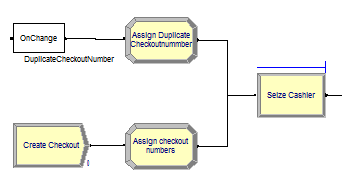
\includegraphics[scale=1]{images/model-description/checkout-creation.PNG}
	\caption{Modeling of the creation of checkouts.}
	\label{fig:createcheckouts}
\end{center}
\end{figure}

The second part of the model is shown in figure \ref{fig:seizeandopen}. When a cashier was seized the checkout moved on to $Active \ Cashiers \ smaller \ than \ 5?$. In this module it is checked whether the shift of the original checkout is finished before the duplicate checkout may move on. If this is not checked it is theoretically possible that both the original checkout and the duplicate checkout are manned. After this module all the associated lanes of the checkout are opened in $Open \ checkout$.

\begin{figure}[h!]
\begin{center}
	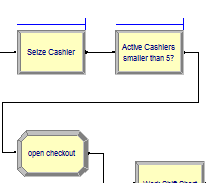
\includegraphics[scale=1]{images/model-description/seize-and-open.PNG}
	\caption{Modeling of the cashier seizing and checkout opening.}
	\label{fig:seizeandopen}
\end{center}
\end{figure}

The next part of the model is shown in figure \ref{fig:workshift}. After that the checkout has opened its associated lanes we first check whether it's a 2 hour or a 4 hour shift. This is necessary because at the start of the simulation (0:00) cashiers from shift 12 are already working and they have only 2 hours left. So these cashiers will go to module $Work \ Shift \ Short$ where a delay of 1 hour and 50 minutes will represent working a shift for the same amount of time. All the other cashiers will go to $Work \ Shift$ where they work for 3 hours and 50 minutes. After these delays the cashiers checkouts reach the module $Trigger \ OnChange$. In this module we trigger the $OnChange$ module mentioned before so that the checkout in this module will be duplicated. Next the cashiers work their remaining 10 minutes in $Work \ Remaining \ Shift$. When the cashier is completely done with his regular shift we decrease the number of active cashiers so that possibly stuck duplicate checkout can continue from the $Active \ Cashiers \ smaller \ than \ 5?$ module we saw before.

\begin{figure}[]
\begin{center}
	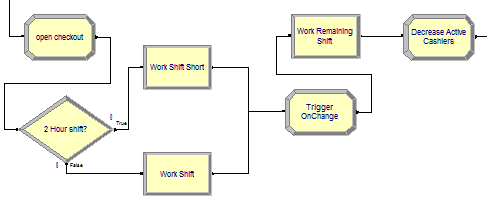
\includegraphics[scale=1]{images/model-description/work-shift.PNG}
	\caption{Modeling of the delay for the cashier working his/her shift.}
	\label{fig:workshift}
\end{center}
\end{figure}

After the regular shift, we have to determine what will happen to the lanes and the cashier. Does he close the lanes and continue working at the checkout till the lanes are empty? Or does another cashier take over and can he go over to restocking the supplies? This is checked in the blocks displayed in figure \ref{fig:determinetakeover}. As you can see, the check whether someone takes over is split into two checks. This is due to a technicality issue: we have a global 1D array with 5 rows. Every row contains a time stamp. This time stamp represents the latest shift which started for that checkout. So in the upper right module $Pump \ Stays \ Open$ we check if the time stamp in the associated row in the array is newer than the expression "TNOW - 3.5", which means is the time stamp less than 3,5 hours old. If not the time stamp is the same as when the shift of the current cashier started and therefore we know the cashier has to close the lanes. If the time stamp is newer it means that another cashier is waiting to take over the shift. The technical problem we have is that for the first 3,5 hours we cannot use this expression, because it will always evaluate to true since there are no negative time stamps. Since shifts only start at whole hours we check if there has past more than 3 hours since the start of the simulation. In the bottom left $Pump \ stays \ Open$ module we just check if the new time stamp is larger or equal to 2, since that is the only shift of cashiers which can take over a checkout before we reach TNOW = 3. 

\begin{figure}[]
\begin{center}
	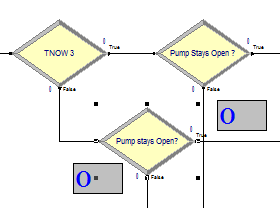
\includegraphics[scale=1]{images/model-description/determine-takeover.PNG}
	\caption{Modeling of the check whether a checkout is taken over.}
	\label{fig:determinetakeover}
\end{center}
\end{figure}

The last part of the cashier management is rather straightforward (figure \ref{closerestockandrelease}): based on the previous decision, the checkout is closed after which the cashier works until the lane and checkout queue are both empty after which he restocks the supplies if less than 10 minutes have passed since the checkout was closed (which is calculated by setting a variable to the current time upon closing and comparing it to current time after the queue is emptied). Or the checkout does not close and the cashier immediately restocks the supplies.
After this the cashier is released and the checkout entity will be disposed.

\begin{figure}[]
\begin{center}
	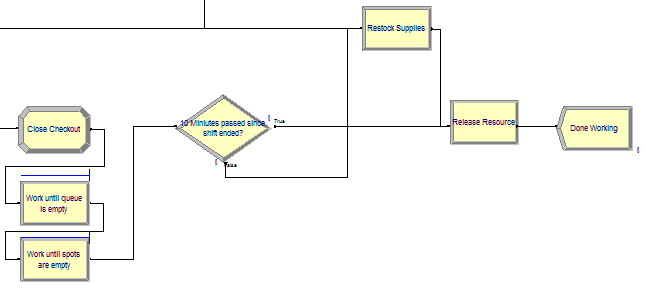
\includegraphics[scale=1]{images/model-description/close-restock-release.PNG}
	\caption{Modeling of the check whether a checkout is taken over.}
	\label{fig:closerestockandrelease}
\end{center}
\end{figure}

	\section{Verification and Validation}

The model was verified and validated.
In verification, the correctness of a model is analysed. 
In validation, a model is compared to the assignment description.

\subsection{Verification}
Sanity checks, an evaluation of Little's formula and an evaluation of the PASTA property have been done in order to verify the correctness of the model. 
All checks have been done by running the model once with a length of 30 days. 

\subsubsection{Sanity checks}

For these sanity checks, the model was run with a schedule where all lanes are always opened.
The total number of arrived vehicles is 61,409.
This is the sum of the number of arrived cars (43,055), the number of arrived cars with trailers (9,186) and the number of arrived trucks (9,168).
It is also verified that vehicles choose the shortest queue on arrival by looking at animation while running the simulation.
Finally, it is confirmed that the cost of this naive schedule is indeed about 3,200 euro a day. 
The total number of worked hours is 3,818.8 for the whole month. 
So 127.3 hours per day, which at a rate of 25 euro per hour comes down to a total cost of 3,182.30 euro.

\subsubsection{Little's formula}
Little's formula states that the average number of jobs in the system, $N$, is equal to the product of the arrival rate $\lambda$ and the average time a job spends in the system, $W$.

For the whole system, we get that the average number of cars arriving per day is 61,409/30 = 2,046.97. 
If we divide this by the number of opening hours per day (24), we get an arrival rate of 2046.97/24 = 85.2903 vehicles per hour.
The average total time a vehicle is in the system is reported to be 0.2713 hours.
The average number of vehicles in the system (WIP) is reported to be 23.1324.
We can see that Little's law holds as:
$$N=\lambda W = 23.2393 = 85.2903\cdot0.2713 \approx 23.1324.$$

\subsubsection{PASTA property}
The PASTA (\textit{Poisson Arrivals See Time Averages}) property holds when the arrival stream is a Poisson process.
From the Arena help, we know that ``If \textit{Schedule} type is Arrival, the \textsc{schedules} element defines a time-dependent schedule of entity arrival rates. (\ldots)
An exponential distribution is used to evenly distribute the \textit{Value} arrivals over each hour."
So the time between events has an exponential distribution.
Poisson processes are processes in which events occur at an average rate (the schedule value) but between the events, the time has an exponential distribution.
We conclude that the arrival of vehicles in our model is a Poisson process and thus that the property holds.
%TODO less bullshit, more testing

\subsection{Validation}
Here, the results of a simulation are compared to the values as provided in the assignment description.
The model was again simulated once with length 30 days and the schedule where all lanes are always opened.

Of the total number of arrived vehicles (61,406), 43,055 where cars. 
This corresponds to 70.1\%, as expected.
Also the number of cars with trailers (9,186, 15.0\%) and the number of trucks (9,168, 14.9\%) correspond to the expected numbers.
Furthermore, the total number of blocked vehicles is 0 in this situation, which shows that the capacity of the fuel station is enough to handle the peak loads.

Finally, a simulation was run with an arrival schedule of 1 arrival every other hour.
This schedule was chosen to make sure no car had to wait.
The average time a car spent in the system was reported to be 0.076 hours, so 4.56 minutes. 
This value is expected from the delays.
Parking the vehicle at the pump, refuelling, cleaning the windows and paying at the cashier can take between 100 seconds (in case of no fuel bought) and 442.5 seconds (in case of 65 liters of fuel bought). 
The expected values for all delays for cars is 222.5 seconds, 3.7 minutes.
The higher average can be explained by the triangular distribution for the waiting time at the cashier. 
The typical value is 90 seconds but it can be much more (270 seconds) and not much less (60 seconds on minimum). 






	\section{Experiment Setup}
As stated before, we are trying to increase profit in the fuel station model.
However, we are limited in ways to do so: we cannot alter the fuel cost, nor is there any way for us to increase customer count.
The only way for us to increase profit, is to lower the cost of fuel station operation, by changing the schedule of the workers. \\
Obviously, it would be cheapest not to have workers at all, but we are to adhere to certain requirements regarding customer satisfaction statistics.
For example, the amount of vehicles that are blocked, by all active lanes being full, may not exceed $1\%$ of all arrived vehicles. \\
This gives rise to some conflicting methods of scheduling.
On the one hand, we can increase income by keeping the blocked percentage as low as possible, conversely, the extra cashiers needed would increase cost as well.
Since we were not given the price of fuel, or any of other services offered, for that matter, we cannot calculate the profit increase.
However, we were given the cost of workers for the fuel station. \\
As a result, we will focus entirely on reducing cost by adjusting the worker schedule as much as possible, even though this might not necessarily yield the optimized profit, depending on fuel and service prices.
As such, in our case, finding the optimal solution to the model means finding the minimal cost schedule, whilst still adhering to the requirements that were imposed.
In this section, we will discuss how we intend to find the optimal solution to our model. \\

In our experiment, we will be using the OptQuest tool that Arena offers natively to find an optimal solution.
Our model contains several decision variables, that we can alter to find the optimal solution.
However, doing so by hand would be very labour intensive indeed.
Moreover, there are constraints that limit our solution space, having to check those would require even more of an effort.
Instead, OptQuest allows us to set bounds to decision variables, and constraints, iterating smartly over the large solution space to maximize an objective variable. \\

As described above, the only decision variables we have are the schedules of the cashiers.
We have 12 shift resources, which define the number of cashiers in each 4-hour shift.
Since there are only 5 cash registers, the number of cashiers in a shift should not exceed 5.
As such, each shift variable should be bounded between 0 and 5.
However, this leads to a rather large solution space, as there are$6^{12}$ possibilities. \\
These are limited, however by several constraints.
First of all, the percentage of vehicles blocked should not exceed 1 percent of the total number of vehicles arrived. \\
Since there are 12 shifts of 4 hours, every shift overlaps with two other shift.
As such, it might occur that there are more cashiers active than there are cash registers.
To combat this problem, and reduce the size of the solution space, we state that the number of workers active at any time should be less than or equal to 5, the number of cash registers. \\
We can then calculate the cost of the given schedule by adding the number of cashiers in every shift, multiplying it by 4, the number of hours in a shift, and multiplying it again by 25, the wage of a worker in euros per hour.
Our goal is then to minimize this cost variable. \\

We will attempt to find a near optimal solution in several steps.
Since the way OptQuest iterates over the data does not guarantee an optimal solution, the best solution found by OptQuest might not be the optimal solution.
As such, instead of simply taking the best solution found by Optquest, we will take several of the best solutions found, and try to optimize these by hand, by removing cashiers from several shifts, whilst ensuring that the requirements are still satisfied. 
		
	\newpage
	\begin{appendix}
	\section{Conceptual Models}

\begin{figure}
\centering
\begin{tikzpicture}

\path[shape=coordinate]
(5,20) coordinate(a11) (5,19.5) coordinate(a12)
(4.75,19.5) coordinate(a13) (5.25,19) coordinate(a14)
(5.75,19.5) coordinate(a15) (5.5,19.5) coordinate(a16)
(5.5,20) coordinate(a17);
\filldraw[fill=blue!20] (a11) -- (a12) -- (a13) -- (a14) -- (a15) -- (a16) -- (a17) -- (a11);

\path[shape=coordinate]
(4,17) coordinate(r11) (4,14) coordinate(r12)
(4.5,14) coordinate(r13) (4.5,17) coordinate(r14);
\filldraw[fill=blue!20] (r11) -- (r12) -- (r13) -- (r14) -- (r11);

\path[shape=coordinate]
(5,17) coordinate(r21) (5,14) coordinate(r22)
(5.5,14) coordinate(r23) (5.5,17) coordinate(r24);
\filldraw[fill=blue!20] (r21) -- (r22) -- (r23) -- (r24) -- (r21);

\path[shape=coordinate]
(6,17) coordinate(r31) (6,14) coordinate(r32)
(6.5,14) coordinate(r33) (6.5,17) coordinate(r34);
\filldraw[fill=blue!20] (r31) -- (r32) -- (r33) -- (r34) -- (r31);

\path[shape=coordinate]
(4,13.5) coordinate(p11) (4,13) coordinate(p12)
(4.5,13) coordinate(p13) (4.5,13.5) coordinate(p14);
\filldraw[fill=blue!20] (p11) -- (p12) -- (p13) -- (p14) -- (p11);

\path[shape=coordinate]
(5,13.5) coordinate(p21) (5,13) coordinate(p22)
(5.5,13) coordinate(p23) (5.5,13.5) coordinate(p24);
\filldraw[fill=blue!20] (p21) -- (p22) -- (p23) -- (p24) -- (p21);

\path[shape=coordinate]
(6,13.5) coordinate(p31) (6,13) coordinate(p32)
(6.5,13) coordinate(p33) (6.5,13.5) coordinate(p34);
\filldraw[fill=blue!20] (p31) -- (p32) -- (p33) -- (p34) -- (p31);

\path[shape=coordinate]
(4,12.5) coordinate(r41) (5,11) coordinate(r42)
(5.5,11) coordinate(r43) (6.5,12.5) coordinate(r44);
\filldraw[fill=blue!20] (r41) -- (r42) -- (r43) -- (r44) -- (r41);

\path[shape=coordinate]
(5,10.5) coordinate(r51) (5,10) coordinate(r52)
(5.5,10) coordinate(r53) (5.5,10.5) coordinate(r54);
\filldraw[fill=blue!20] (r51) -- (r52) -- (r53) -- (r54) -- (r51);

\node[draw=none] at (5.25,20.5) (arr) {Arrive};
\node[draw=none](t1) at (1,19.5){
\begin{tabular}{|l|l|l|}
\hline
\multicolumn{3}{|l|}{Arrivals} \\
\hline
Car     & 70\%  & 1 \\
Trailer & 15\%  & 2 \\
Truck   & 15\%  & 3 \\
\hline
\end{tabular}};
\node[draw=none](t2) at (9,19.5){
\begin{tabular}{l}
Leave when full \\
(at most 1\%)
\end{tabular}};
\node[draw=none](t3) at (1,15.5){
\begin{tabular}{l}
Lines \\
-cap: 16
\end{tabular}};
\node[draw=none](t4) at (1,13.25){
\begin{tabular}{|l|}
\hline
Pump \\
\hline
-30-45s park \\
-pump: 40/130 $\frac{L}{m}$ \\
-10-30s drive \\
\hline
\end{tabular}};
\node[draw=none](t5) at (9,11.75){
\begin{tabular}{|l|}
\hline
Wait \\
\hline
-3 × 1 after pump \\
-2 in between \\
-1 at cashier \\
\hline
\end{tabular}};
\node[draw=none](t6) at (1,10.25){
\begin{tabular}{l}
Cashier \\
-90s-4.5 minutes
\end{tabular}};
\node[draw=none](t7) at (5.25,7.5){
\begin{tabular}{|l|}
\hline
Shifts \\
\hline
-25 euro per hour \\
-4 hours every 2 hours \\
-close $\rightarrow$ serve until empty\\
\hline
\end{tabular}};
\node[draw=none](k9) at (9,15.5){
\begin{tabular}{l}
0...5
\end{tabular}};

\draw[dotted, shorten >= .3cm] (t1) -- (a13);
\draw[dotted, shorten >= .3cm] (t2) -- (a15);
\draw[dotted, shorten >= .3cm] (t3) -- (t3 -| r11);
\draw[dotted, shorten >= .3cm] (t4) -- (t4 -| p11);
\draw[dotted] (t5) -- (t5 -| r44);
\draw[dotted, shorten >= .3cm] (t6) -- (t6 -| r51);

\draw[<->,double, shorten >= .3cm, shorten <= .3cm] (k9) -- (k9 -| r34);

\end{tikzpicture}
\caption{Conceptual model Nicky Advokaat}
\end{figure}

\textbf{Problems of the model}
\begin{enumerate}
\item There is no clear flow between the states.
\item The number of queues is incorrect.
\item The action cleans windows is missing from the pump actions.
\end{enumerate}

\newpage

\begin{figure}
\centering
\begin{tikzpicture}[
place/.style={
rectangle,
minimum size=6mm,
semithick,
draw=black,
fill=blue!20
},
title/.style={
draw=none,
fill=none,
color=gray,
anchor=west
},
ptext/.style={
draw=none,
fill=none,
color=black
},
superplace/.style={
matrix of nodes,
nodes=place,
row 1/.style={
    nodes=title
},
row sep=0.5em,
column sep={3em,between origins},
matrix anchor=north,
rectangle,
semithick,
draw=black,
fill=orange!20
}]

\matrix[row sep = 3em] (mat) {
\node [draw=none] (track) {Trucks}; &
\node [draw=none] (cave) {Cars + trailer}; &
\node [draw=none] (car) {Cars}; &\\

&\node [place] (enter) {Enter station}; & & \\

&\node [place] (choose) {Choose (shortest) lane}; & & \node [draw=none](t1) {
\begin{tabular}{l}
Leave if all \\ lanes blocked
\end{tabular}}; \\
&\node [place] (queue) {Queue}; & & \\
&\node [place] (getf) {Get fuel}; & & \node[draw=none] (t2) {and clean windows}; \\
&\node [place] (queue2) {Queue}; & & \\
&\node [place] (pay) {Pay at cashier}; & & \\
&\node [place] (leave) {Leave}; & & \\
};

\node [draw=none,below =of mat] {This does not include leaving/taking over shifts};

\draw[->,thick] (car) -- (enter.north east);
\draw[->,thick] (cave) -- (enter.north);
\draw[->,thick] (track) -- (enter.north west);

\draw[->,thick] (enter) -- (choose);
\draw[->,thick] (choose) -- (queue);
\draw[->,thick] (queue) -- (getf);
\draw[->,thick] (getf) -- (queue2);
\draw[->,thick] (queue2) -- (pay);
\draw[->,thick] (pay) -- (leave);

\draw[->,thick] (choose) -- (t1);
\draw[->,thick] (t2) -- (getf);

\end{tikzpicture}
\caption{Conceptual model Robbert Jongeling}
\end{figure}

\textbf{Problems of the model}
\begin{enumerate}
\item The arrival percentages are missing.
\item The number of queues are missing.
\item The different actions in the fuel state are missing.
\item Information about the fuel times and waiting times is missing.
\end{enumerate}

\newpage

\begin{figure}
\centering
\begin{tikzpicture}[
place/.style={
rectangle,
minimum size=6mm,
semithick,
draw=black,
fill=blue!20
},
title/.style={
draw=none,
fill=none,
color=gray,
anchor=east
},
ptext/.style={
draw=none,
fill=none,
color=black
},
superplace/.style={
matrix of nodes,
nodes=place,
row 1/.style={
    nodes=title
},
row sep=0.5em,
column sep={3em,between origins},
matrix anchor=north,
rectangle,
semithick,
draw=black,
fill=orange!20
}]

\node [draw=none] (cave) {};
\node [place,below =of cave] (arr) {Arriving};

\matrix [superplace,below of=arr](queueing){
    Queueing & & &\\
    & |(selq)| Select Queue & &\\
    & & &\\
    & & &\\
    & & &\\
    |[label=below:$1$,inner sep=0](q1)|\rotatebox{90}{\tbsep} & |[label=below:$2$,inner sep=0](q2)|\rotatebox{90}{\tbsep} &  & |[label=below:$15$,inner sep=0](q15)|\rotatebox{90}{\tbsep} \\
};

\node [draw=none, left =of queueing] (block) {};

\matrix [superplace,below =of queueing](refueling){
    Refueling\\
    |(park)| Parking\\
    |(ref)| Refueling\\
    |(clean)| Clean windows\\
};

\matrix [superplace,below =of refueling](caque){
    Cashier \\
     |[label=below:$1$,inner sep=0](c1)|\rotatebox{90}{\tbsep} & |[label=below:$2$,inner sep=0](c2)|\rotatebox{90}{\tbsep} &  & |[label=below:$5$,inner sep=0](c5)|\rotatebox{90}{\tbsep} \\
};

\node [place,right =of caque] (pay) {Paying};
\node [draw=none, right =of pay] (lea) {Vehicle leaves};

\node [draw=none] at (7,-0.5) (t1) {
\begin{tabular}{|l | l|}
\hline
\multicolumn{2}{|l|}{Vehicles}\\
\hline
70\% & Car \\ 15\% & Car with trailer \\ 15\% & Truck \\
\hline
\end{tabular}};
\node [draw=none] at (7,-3.8)(t2) {
\begin{tabular}{|l|}
\hline
Vehicles select shortest open queue\\
\hline
At most 1\% blocked\\
\hline
\end{tabular}};
\node [draw=none] at (7,-6)(t3) {
\begin{tabular}{|l|l|}
\hline
\multicolumn{2}{|l|}{Max waiting time} \\
\hline
Car & \multirow{2}{*}{30 min (1800 sec)} \\
(with trailer) & \\
Truck & 45 min (2700 sec) \\
\hline
\end{tabular}};
\node [draw=none] at (5.6,-9.2)(t4) {
\begin{tabular}{|l|}
\hline
30-45 seconds \\
\hline
\end{tabular}};
\node [draw=none] at (7,-10.7)(t5) {
\begin{tabular}{|l|l|}
\hline
\multicolumn{2}{|l|}{Time, depends on fuel amount} \\
\hline
Car & \multirow{2}{*}{fuel / 40 min} \\
(with trailer) & \\
Truck & fuel / 130 min \\
\hline
\end{tabular}};
\node [draw=none] at (5.6,-12.2)(t6) {
\begin{tabular}{|l|}
\hline
10-30 seconds \\
\hline
\end{tabular}};
\node [draw=none] at (7,-14.2)(t7) {
\begin{tabular}{|l|}
\hline
Pick cashier queue corresponding\\
to lane (1-3$\rightarrow$1, 4-6$\rightarrow$2, etc) \\
\hline
\end{tabular}};
\node [draw=none] at (6.5,-17.3)(t8) {
\begin{tabular}{|l|}
\hline
Typically 90 seconds\\
Maximum 4.5 min (270 sec) \\
\hline
\end{tabular}};

\draw[->,thick] (cave) --  coordinate[midway](m)(arr.north);

\draw[->,thick] (arr.south -| selq.north) -- (selq.north);

\draw[->,thick] (selq.west) -- (selq.west -| block) node[midway,below,draw=none] {Blocked};
\draw[->,thick] (pay.east) -- (lea.west);

\draw[->,thick] (selq.south -| q1.north) -| (q1.north);
\draw[->,thick] (selq.south -| q2.north) -- (q2.north);
\draw[->,thick] (selq.east) -| (q15.north);

\draw[->,thick] (queueing.south) -- (refueling.north);
\draw[->,thick] (refueling.south) -- (caque.north);
\draw[->,thick] (caque.east |- pay.west) -- (pay.west);

\draw[dotted, shorten >= .3cm, shorten <= .3cm] (q2) -- (q15);

\draw[dotted,semithick] (t1.west |- m) -- (m);
\draw[dotted,thick,bend right=45] (t2.north west) to (selq.north east);
\draw[dotted,semithick] (t3.west |- q15) -- (q15);

\draw[dotted,thick] (t4.west) -- (park.east);
\draw[dotted,semithick] (t5.west |- ref) -- (ref);
\draw[dotted,semithick] (t6.west |- clean) -- (clean);

\draw[dotted,semithick] (t7.west -| caque.east) -- (t7);
\draw[dotted,semithick] (t8.north -| pay) -- (pay);

\draw[dotted, shorten >= .3cm, shorten <= .3cm] (c2.east) -- (c5.west);

\end{tikzpicture}
\caption{Conceptual model Bram Kohl}
\end{figure}

\textbf{Problems of the model}
\begin{enumerate}
\item There were no clear problems with this model.
\end{enumerate}

\newpage

\begin{figure}
\centering
\begin{tikzpicture}[
place/.style={
rectangle,
minimum size=6mm,
semithick,
draw=black,
fill=blue!20
},
title/.style={
draw=none,
fill=none,
color=gray,
anchor=west
},
ptext/.style={
draw=none,
fill=none,
color=black
},
superplace/.style={
matrix of nodes,
nodes=place,
row 1/.style={
    nodes=title
},
row sep=0.5em,
column sep={3em,between origins},
matrix anchor=north,
rectangle,
semithick,
draw=black,
fill=orange!20
}]
\node [draw=none] (cave) {Car + Vehicle};
\node [draw=none,left =of cave] (car) {Car};
\node [draw=none,right =of cave] (track) {Truck};

\node [place,below =of cave] (arr) {Arriving};

\matrix [superplace,below of=arr](queueing){
    Queueing & & & &\\
    & & |(selq)| Select Queue & &\\
    & & & &\\
    & & & &\\
    & & & &\\
    & |[label=below:$1$,inner sep=0](q1)|\rotatebox{90}{\tbsep} & |[label=below:$2$,inner sep=0](q2)|\rotatebox{90}{\tbsep} &  & |[label=below:$15$,inner sep=0](q15)|\rotatebox{90}{\tbsep} \\
};

\node [place,below =of queueing] (pump) {Pump};
\node [place,below =of pump] (queue) {Queue};
\node [place,below =of queue] (pay) {Pay};
\node [place,below =of pay] (leave) {Leave};

\node [draw=none] at (7,-1.5)(t1) {
\begin{tabular}{l}
70\% Car \\ 15\% Car with trailer \\ 15\% Truck
\end{tabular}};
\node [draw=none] at (7,-3.8)(t2) {Select shortest queue};
\node [draw=none] at (7,-5.5)(t3) {
\begin{tabular}{l}
Staffing costs \\ Cashier 25,- per hour
\end{tabular}};
\node [draw=none, right=2cm of pump](t4) {
\begin{tabular}{l}
Park the car: 30-45 sec \\ Refuels, clean the windows,\\ start again: 10-30s
\end{tabular}};
\node [draw=none, right=2cm of pay](t5) {
\begin{tabular}{l}
Avg transaction time: 90s \\ Max transaction time: 270s
\end{tabular}};

\node [draw=none, below=of leave](t6) {
\begin{tabular}{l l}
Car(with trailer) &avg at most 30 min \\ Truck &avg at most 45 min
\end{tabular}};

\draw[->,thick] (car) -- (arr.north west);
\draw[->,thick] (cave) -- (arr.north);
\draw[->,thick] (track) -- (arr.north east);

\draw[->,thick] (arr.south -| selq.north) -- (selq.north);

\draw[->,thick] (selq.south -| q1.north) -- (q1.north);
\draw[->,thick] (selq.south -| q2.north) -- (q2.north);
\draw[->,thick] (selq.east) -| (q15.north);

\draw[dotted, shorten >= .5cm, shorten <= .5cm] (q2) -- (q15);

\draw[->,thick] (queueing) -- (pump);
\draw[->,thick] (pump) -- (queue);
\draw[->,thick] (queue) -- (pay);
\draw[->,thick] (pay) -- (leave);

\draw[->,thick, shorten >= .5cm] (t1.west |- arr) -- (arr);
\draw[->,thick, shorten >= 2cm] (t2.west |- selq) -- (selq);
\draw[->,thick, shorten >= .5cm] (t3.west |- queueing) -- (queueing);
\draw[->,thick, shorten >= .5cm] (t4) -- (pump);
\draw[->,thick, shorten >= .5cm] (t5) -- (pay);

\end{tikzpicture}
\caption{Conceptual model Jasper Selman}
\end{figure}

\textbf{Problems of the model}
\begin{enumerate}
\item Misses info in the pump state about the refueling.
\item It is not possible for a car to get blocked and therefore not go into a queue.
\end{enumerate}

\newpage

\begin{figure}
\centering
\begin{tikzpicture}[
place/.style={
rectangle,
minimum size=6mm,
semithick,
draw=black,
fill=blue!20
}]

\matrix[row sep=4em,column sep={10em,between origins}]{
                            &   \node[draw=none] (s) {};                \\
                            &   \node[place] (arr) {Arrival};           \\
\node[place] (l1) {Leave};  &   \node[place] (selq) {Select queue};     \\
                            &   \node[place] (queue) {In queue};        \\
                            &   \node[place] (ref) {Refuel and clean windows};            \\
                            &   \node[place] (cash) {Cashier queue};    \\
                            &   \node[place] (pay) {Pay};               \\
                            &   \node[place] (l2) {Leave};              \\
};

\node[draw=none](t1) at (8,6){
\begin{tabular}{|l|l|l|}
\hline
Vehicle type & Frequency & Length\\
\hline
Car     & 70\%  & 1 \\
Trailer & 15\%  & 2 \\
Truck   & 15\%  & 3 \\
\hline
\end{tabular}};
\node[draw=none](t2) at (8,1.3){
\begin{tabular}{|l|}
\hline
Queue space: 16 \\
\hline
\end{tabular}};
\node [draw=none] at (8,-1)(t3) {
\begin{tabular}{|l|l|}
\hline
Park time & 30-45 sec \\
\hline
\hline
Type & Refuel time \\
\hline
Car (+trailer) & $40 \frac{L}{min}$ \\
Truck & $130 \frac{L}{min}$ \\
\hline
\hline
Drive off & 10-30 sec \\
\hline
\end{tabular}};
\node[draw=none](t4) at (8,-5){
\begin{tabular}{|l|}
\hline
Typically 90s \\
up to 4.5 min \\
\hline
\end{tabular}};
\node[draw=none](t5) at (8,-8){
\begin{tabular}{|l|}
\hline
Staff \\
\hline
-25 euro per hour \\
-4 hour shifts \\
\hline
\end{tabular}};

\draw[->,thick] (s) -- (arr);
\draw[->,thick] (arr) -- (selq);
\draw[->,thick] (selq) -- (l1) node[draw=none,midway,above]{full};
\draw[->,thick] (selq) -- (queue) node[draw=none,midway,left]{Pick shortest queue};
\draw[->,thick] (queue) -- (ref);
\draw[->,thick] (ref) -- (cash);
\draw[->,thick] (cash) -- (pay);
\draw[->,thick] (pay) -- (l2);

\draw[dotted,semithick] (t1.west |- arr) -- (arr);
\draw[dotted,semithick] (t2.west |- queue) -- (queue);
\draw[dotted,semithick] (t3.west |- ref) -- (ref);
\draw[dotted,semithick] (t4.west |- pay) -- (pay);

\end{tikzpicture}
\caption{Conceptual model Ramon de Vaan}
\end{figure} 

\textbf{Problems of the model}
\begin{enumerate}
\item Misses info about the cashier queue.
\item Misses the percentage of blocked vehicles.
\item Misses the number of queues.
\end{enumerate}
	\newpage
	\section{Appendix Input Analysis}\label{app:inputanalysis}
\begin{figure}[h]
	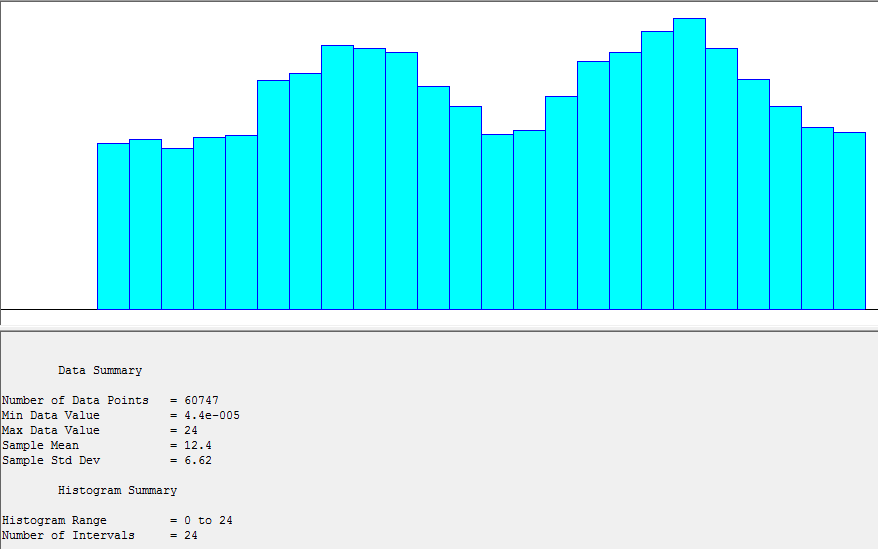
\includegraphics[width=\textwidth]{images/histogram-arrivals.PNG}
	\caption{Histogram of arrival times, each of the 24 intervals represents one hour.}
	\label{fig:histogram-arrivals}
\end{figure}

\begin{table}[h]
	\centering
	\begin{tabular}{r | l}
		Function  &     Sq Error\\
		\hline
		Beta       &  0.000889\\
		Uniform     & 0.00141\\
		Normal       &0.00507\\
		Gamma        &0.00703\\
		Erlang       &0.00712\\
		Triangular   &0.00915\\
		Lognormal    &0.0122\\
		Exponential  &0.0143\\
		Weibull      &0.107	
	\end{tabular}
	\caption{Fit all summary of Arena Input Analyzer on Arrivals\_(13).dst}
	\label{tab:fitallarrivals}
\end{table}

Figure \ref{fig:histogram-inter-arrivals} shows a histogram of the time difference between successive arrivals. This data fits a Poisson distribution with mean \todo[inline]{Poisson mean}

\begin{figure}[h]
	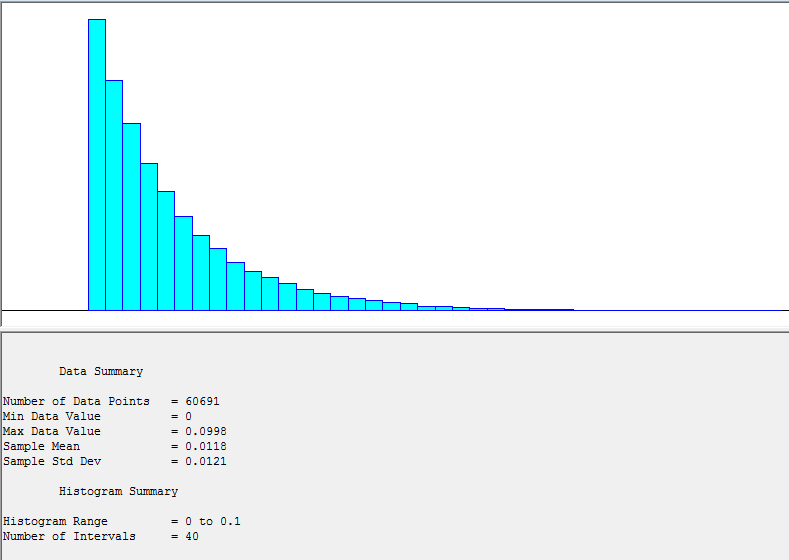
\includegraphics[width=\textwidth]{images/histogram-interarrivaltimes.PNG}
	\caption{Histogram of inter arrival times, 40 intervals over the range 0 - 0.1 hours.}
	\label{fig:histogram-inter-arrivals}
\end{figure}

\begin{figure}[h]
	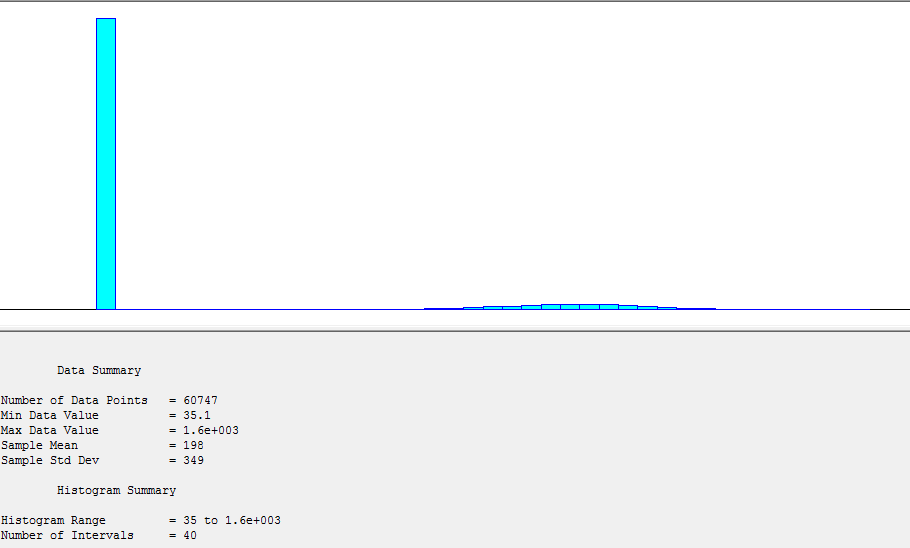
\includegraphics[width=\textwidth]{images/histogram-amounts-unfiltered.PNG}
	\caption{Histogram of used fuel amounts, 40 intervals, on the raw data}
	\label{fig:histogram-amounts-unfiltered}
\end{figure}

\begin{figure}[h]
	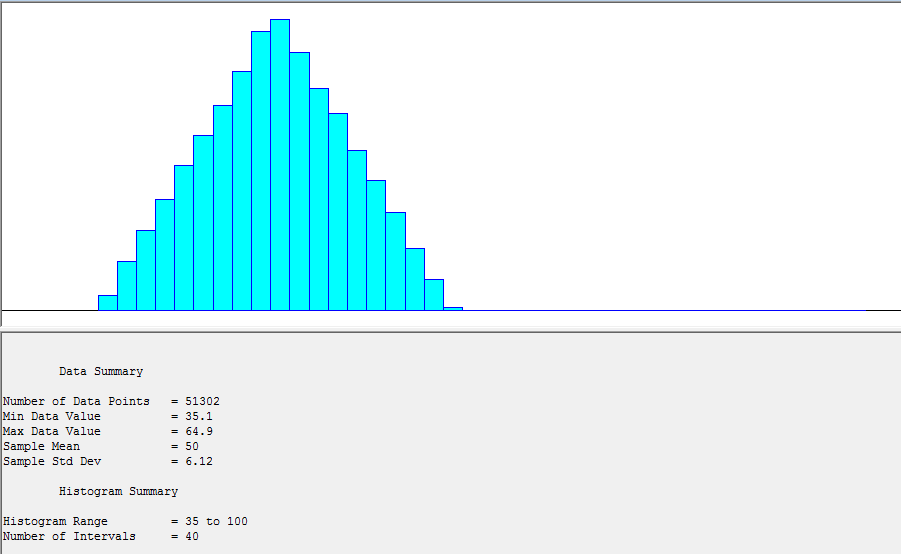
\includegraphics[width=\textwidth]{images/histogram-amounts-filtered.PNG}
	\caption{Histogram of used fuel amounts, 40 intervals, when maximum data value was set to 100 litres.}
	\label{fig:histogram-amounts-filtered}
\end{figure}

\begin{figure}[h]
	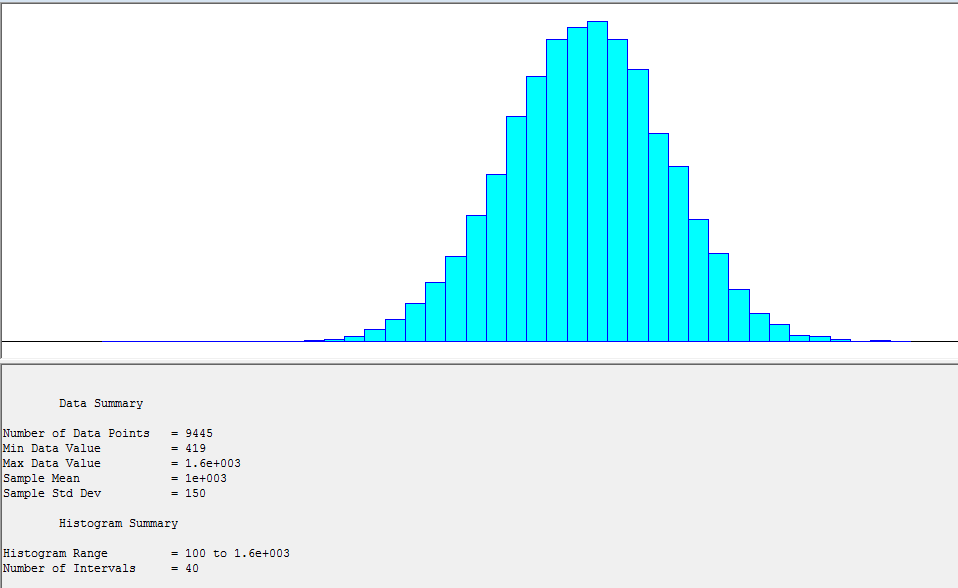
\includegraphics[width=\textwidth]{images/histogram-amounts-filtered-min100.PNG}
	\caption{Histogram of used fuel amounts, 40 intervals, when minimum data value was set to 100 litres.}
	\label{fig:histogram-amounts-filtered-trucks}
\end{figure}

\begin{table}[h]
	\parbox{.3\linewidth}{
		\centering
		\begin{tabular}{r | l}
			Function  &     Sq Error\\
			\hline
			Lognormal    &0.0976\\
			Weibull      &0.118\\
			Beta         &0.226\\
			Gamma        &0.285\\
			Exponential  &0.473\\
			Erlang       &0.473\\
			Normal       &0.668\\
			Triangular   &0.679\\
			Uniform      &0.69\\
		\end{tabular}
		\caption{Fit all summary of Arena Input Analyzer on Amounts\_(13).dst}
		\label{fitallamountsunfiltered}
	}
	\parbox{.05\linewidth}{\ }
	\parbox{.3\linewidth}{
		\centering
		\begin{tabular}{r | l}
			Function  &     Sq Error\\
			\hline
			Normal       &0.000575\\
			Weibull      &0.000587\\
			Beta         &0.00239\\
			Erlang       &0.00387\\
			Gamma        &0.00411\\
			Lognormal    &0.00888\\
			Triangular   &0.0277\\
			Exponential  &0.0397\\
			Uniform      &0.0471\\
			
		\end{tabular}
		\caption{Fit all summary of Arena Input Analyzer on Amounts\_(13).dst with maximum amount set to 100}
		\label{fitallamountsfilteredcars}
	}
	\parbox{.05\linewidth}{\ }
	\parbox{.3\linewidth}{
		\centering
		\begin{tabular}{r | l}
			Function  &     Sq Error\\
			\hline
			Normal       &4.18e-005\\
			Weibull      &0.00062\\
			Lognormal    &0.00123\\
			Erlang       &0.00215\\
			Gamma        &0.00219\\
			Beta         &0.00276\\
			Triangular   &0.0201\\
			Uniform      &0.0454\\
			Exponential  &0.0594
			
		\end{tabular}
		\caption{Fit all summary of Arena Input Analyzer on Amounts\_(13).dst with minimum amount set to 100}
		\label{fitallamountsfilteredtrucks}
	}
	\caption{Summaries of \textit{Fit all} of Arena Input Analyzer, all with 40 intervals}
	\label{tab:fitallamounts}
\end{table}
	\newpage
	\section{Appendix Simulation Model Description}\label{app:modeldescription}
\begin{figure}[H!]
	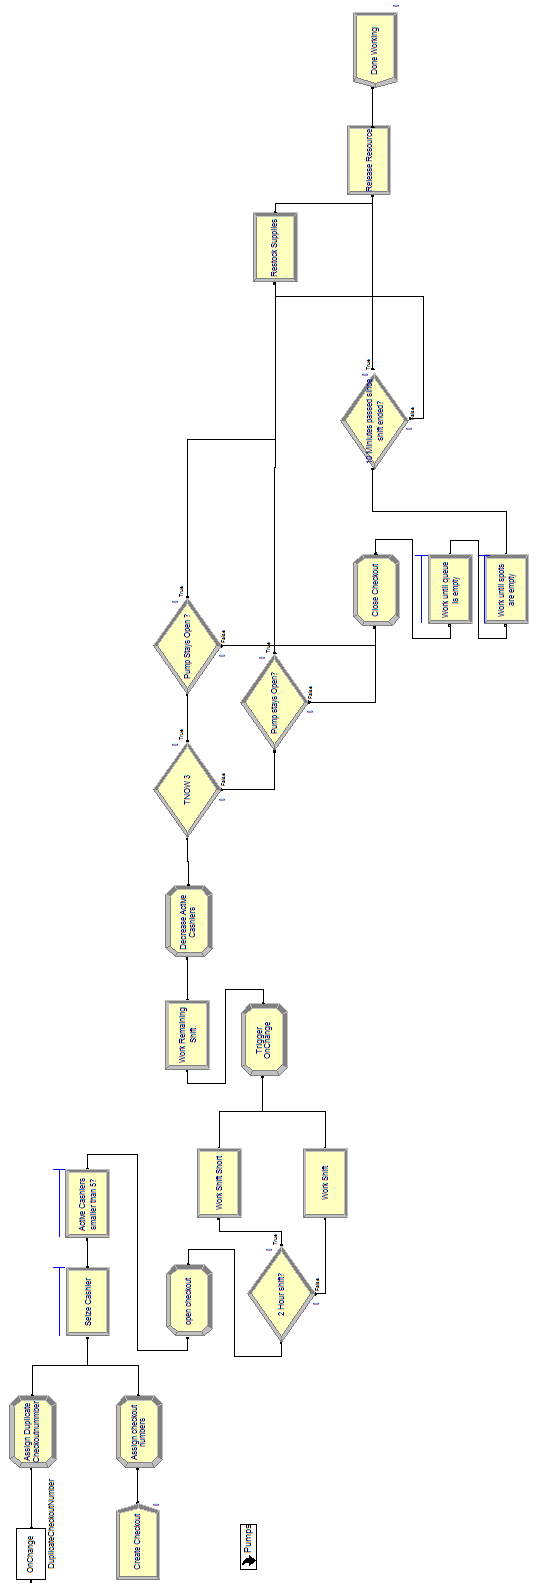
\includegraphics[scale=0.3]{images/model-description/model-cashier-management.PNG}
	\caption{Arena simulation model of the cashier management.}
	\label{fig:model-cashier}
\end{figure}
	\end{appendix}
\end{document}
